\documentclass[class=scrartcl,crop=false]{standalone}

\usepackage{../style/smtikz}

\begin{document}

\section{SMTikZ}

This node is not square:

\begin{center}
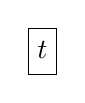
\begin{tikzpicture}
    \node [draw] {$t\mathstrut$};
\end{tikzpicture}
\end{center}

This node is square:

\begin{center}
    \begin{tikzpicture}
        \node [draw,square] {$t\mathstrut$};
    \end{tikzpicture}
    \end{center}


An NFA box:

\begin{center}
\begin{tikzpicture}
    \pic (a)  {tbox={2}{1/2/}};
\end{tikzpicture}
\end{center}

An NBA box:

\begin{center}
\begin{tikzpicture}
    \pic {tbox={2}{2/1/dot, 1/1/dot}};
\end{tikzpicture}
\end{center}

A game arena:

\begin{center}
\begin{tikzpicture}
[scale=0.6,node distance=2cm]
\node (5) [squarepos] {5};

\node (1) [squarepos,below of=5] {1};
\node (2) [squarepos,below of=1] {2};

\node (3) [roundpos, left of=1] {3};
\node (4) [roundpos, right of=1] {4};

%        \node (6) [squarepos,below of=2] {6};


\path [draw,->,semithick,>=latex]
(3) edge (1)
(3) edge (5)
(1) edge (4)
(4) edge (2)
(2) edge (3)
(4) edge (5)
%            (6) edge (3)
%            (6) edge (4)
;

\end{tikzpicture}
\end{center}

\end{document}
